\chapter{Appendix}
\section{Definition of Domain Specific Languages (DSL)}
\par
%A domain-specific language (DSL), in contrast to general purpose languages, is specialized in a selected application domain.​ Only typical tasks from this domain can often be solved with DSL, but due to highly specialized language elements with little effort and using the natural concepts from the application domain.
\par
The source code of such languages can be later translated automatically into the source code of a general purpose language like Java, C\#, C++ or other. The advantage is that the language scope of the DSL because of the specialization to a domain is much smaller, in comparison to a general purpose language. In extreme cases, instead of the programmer the application expert could write the required program [01]. %TODO quote
\begin{figure}[h]
	\centering
	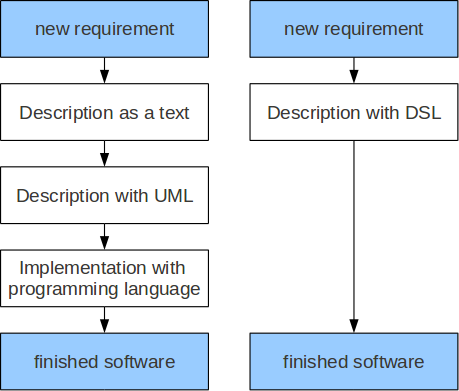
\includegraphics[width=0.7\textwidth]{pics/appendix/dsl.png}
	\caption{Comparison of the development process with a DSL and a general purpose language.  \label{fig:dsl}}	
\end{figure}
\par
For the development, maintenance and continuous adaptation of the DSL, experts are required. The knowledge of these people needs to be extended. If necessary, an external service may be used [01].
%TODO quote

\section{Definition of Ontology}
Ontologies enable or improve the communication between computer systems, computer systems and humans, but also between people in a given domain. Ontology consists of mostly a defined basic vocabulary, definitions and entities that build on this basic vocabulary and a description of the existing relations among each other. The following figure \ref{fig:semiotic_triangle} illustrates the interaction between words (or more generally symbols), concepts and real things in the world [02]. %TODO quote
\begin{figure}[h]
	\centering
	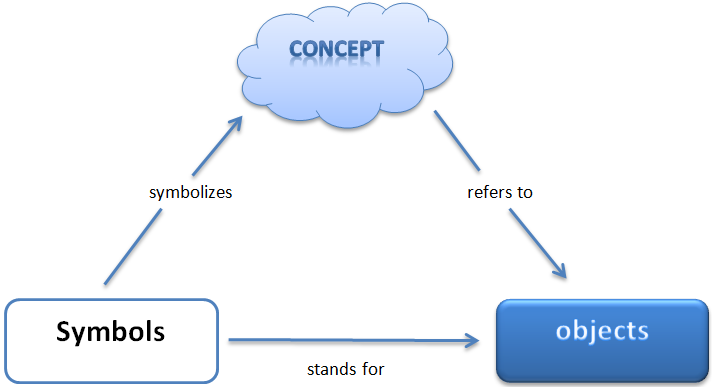
\includegraphics[width=0.7\textwidth]{pics/appendix/onto.png}
	\caption{Semiotic triangle \label{fig:semiotic_triangle}}	
\end{figure}
\par
The formal logic that ontology are based on defines rules that can be used to reason about terms and symbols. This reasoning is always correct and independent of interpretation or observation. Science recognizes this, using logic to derive and state hypotheses, but not to test or verify them. Testing requires experiments and observation, involving a non-trivial and imperfect interpretation between theoretical terms and real world phenomena, known as experiment design. Logical “proofs” say nothing about the real world, they only deal with dependencies between language elements [02]. %TODO quote

\section{Definition of Declarative programming language}
\par
Declarative programming is a programming paradigm in which the description of the problem is in the foreground. The solution is then determined automatically. Declarative programming languages have higher levels of expression and abstraction than most other programming paradigms. Not only does declarative programming reduce source code — it also prevents many common bugs that cripple any large C++ or Java development project [03]. 
%TODO quote

\par
Declarative programming languages are for example:
\begin{itemize}
	\item functional languages (e.g. LISP, ML, Miranda, Gofer, Haskell, Erlang)
	\item logical languages (e.g. Prolog)
	\item transformation languages (e.g. XSLT)
	\item query languages (e.g. SQL)
	\item etc...
\end{itemize}

\par
In contrast to imperative programming, in which the focus is on HOW you want to calculate, in the declarative programming the focus is on WHAT you want to calculate. This can be seen in the following example, which shows a short implementation of quicksort, written in the declarative programming language Haskell. The example is taken from [4]. %TODO quote
\begin{lstlisting}[language=Haskell]
 quicksort [] = []
 quicksort (x:xs) = quicksort [n | n<-xs, n<x] ++ [x] ++ quicksort [n | n<-xs, n>=x]
\end{lstlisting}
The programmer describes what the program have to do with a command, so how to deal with input, the calculation process is not of interest. The calculations are then carried out by manipulating values.
\par
The programs written in declarative programming languages are often shorter than comparable imperative programs. There are no side effects because of referential transparency. Programs are thus partially evaluated and allow the treatment of infinite data structures for example [03].
%TODO quote
\section{Model paradigms}
\subsection{System Dynamics}
\par
System Dynamics (SD) is a common dynamic modelling paradigm within the ecological and environmental research communities. A SD model consists of compartments (stocks, levels, storages) connected by flows, with subsidiary variables for representing parameters and intermediate variables, and influence arrows to show which compartments and variables are used in the calculation of flows and other variables. Essentially, SD is a cosmetic language for defining differential- or difference-equation models: differential equations if the equations are taken to define continuous change; difference equations if the time step is taken to be unity [05]. %TODO quote

\section{Grammar of the first DSL draft}
\par
The first DSL draft had the goal to be able to represent the Similie Bank Tutorial \autocite{dsl:similie_tutorial_bank} textually. Its grammar looked like the following:
\begin{lstlisting}
Model:
Model_Description;

Model_Description :
'Model' name=ID ':'    Declaration+=Declaration*;

Declaration:
Definition |    Conjunction

Definition:
Container |    Variable |    Flow ;

Container:
'Container' Type_def name=ID '=' exp=Expression ';' ;

Variable:
'Variable' Type_def name=ID '=' exp=Expression ';' ;

Flow:
'FlowIN' Type_def name=ID 'IN' name2=Container '=' exp=Expression ';' |
'FlowOUT' Type_def name=ID 'FROM' name2=Container '=' exp=Expression ';' ;

Conjunction:
'Conjunction' from=ID '--' to=ID ';' ;

Type_def:
typedef=ID ;

Expression :
Addition;

Addition returns Expression:
Multiplication (({Plus.left=current} '+' | {Minus.left=current} '-') right=Multiplication)*;

Multiplication returns Expression:
PrimaryExpression (({Multi.left=current} '*' | {Div.left=current} '/') right=PrimaryExpression)*;

PrimaryExpression returns Expression:
'(' Expression ')' |    {NumberLiteral} value=NUMBER ;

terminal NUMBER returns ecore::EBigDecimal:
('0'..'9')* ('.' ('0'..'9')+)?;
\end{lstlisting}

\section{Predator-Prey model with our second DSL draft}
\par
A predator-prey model from \autocite{dsl:dynamo} written with our second DSL draft. It is not complete, but it shows that the code is already bloated.
\newline
\begin{lstlisting}
//**************************************
//***Begin of Declarative Part**********
//**************************************
describe DeerPopulation depends on DeerPopulation_old, DeerWR, DeerPreyRate , timestep as
   DeerPopulation_old + timestep * ( ??? )
describe A depends on  as 800000;
describe DeerFrequency depends A , DeerPopulation as
   DeerPopulation / A  

describe fodderAmount depends on fodderAmount_old , timestep,newFodderRate , fodderEatenRate as
   ???

describe fodderCapacity depends on timestep as 350000

describe predatorPopulation depends on predatorPopulation_old , timestep , predatorGrowingRate, predatorDecreasingRate as
   ???

describe predatorDecreasingRate depends on timestep as 0,2

describe deerGrowingF depends on fodderPerDeer as  DISKRETE_FUNKTION[fodderPerDeer]

describe fodderPerDeer depends on  fodderAmount, DeerPopulation, timestep as
   fodderAmount / DeerPopulation

describe deerGrowingRate depends on deerGrowingF , DeerPopulation , timestep as
   deerGrowingF * DeerPopulation ;       

describe DeerPreyRate depends on
  ???

//**************************************
//***Begin of Imperative Part***********
//**************************************
run simulation from 1907 ... 1950
init
   DeerPopulation = 4000
   fodderAmount = 350000
   predatorPopulation = 8000  

   fodderPerDeer_new = fodderPerDeer ( fodderAmount , DeerPopulation )
   DeerPreyRate_new = ???
   deerGrowingF_new = deerGrowingF (fodderPerDeer )
   deerGrowingRate_new = deerGrowingRate( deerGrowingF_new, DeerPopulation)
   DeerPopulation = DeerPopulation(DeerPopulation , deerGrowingRate_new , DeerPreyRate)
\end{lstlisting}

















 







